\chapter{Determinizm procesu trenowania}
\thispagestyle{chapterBeginStyle}

\section{Opis determinizmu}

Algorytm deterministyczny może zostać zdefiniowany poprzez określenie sposobu zmiany stanów maszyny, która wykonuje algorytm. Algorytm jest deterministyczny jeśli dla pewnego stanu i pewnych danych wejściowych istnieje dokładnie jedna dopuszczalna zmiana stanu. W praktyce oznacza to, że zaczynając od pewnego stanu początkowego, można dokładnie określić kolejne stany maszyny wykonującej algorytm.

\section{Determinizm sieci neuronowych}

W kontekście sieci neuronowych, determinizm jest wymagany do zachowania powtarzalności eksperymentów. Posiadając ustalony zbiór treningowy, opis architektury sieci neuronowej oraz algorytm przeprowadzenia procesu trenowania, algorytm powinien za każdym razem zwracać ten sam zbiór parametrów sieci neuronowej. W przypadku trenowania sieci neuronowych na procesorach CPU (ang. central processing unit) wystarczy ustawić wartość ziarna generatora liczb pseudolosowych. Podczas trenowania z użyciem procesora GPU (ang. graphics processing unit), należy wprowadzić kilka dodatkowych zmian, które ograniczają optymalizacje prędkości trenowania, ale zapewniają powtarzalność wyników.

\section{Implementacja determinizmu}
\begin{minted}{python}
import torch                                   # sieci neuronowe
import numpy as np                             # operacje na macierzach
import random                                  # generatory pseudolosowe
import os                                      # modul komunikacji z systemem


def set_seed(seed):
    torch.manual_seed(seed)                    # ustawienie ziarna biblioteki torch
    torch.cuda.manual_seed_all(seed)           # ustawienie ziarna biblioteki cuda
    torch.backends.cudnn.deterministic = True  # deterministyczne algorytmy cudnn
    torch.backends.cudnn.benchmark = False     # stały zbiór algorytmów cudnn
    np.random.seed(seed)                       # ustawienie ziarna biblioteki numpy
    random.seed(seed)                          # ustawienie ziarna biblioteki random
    os.environ['PYTHONHASHSEED'] = str(seed)   # ustawienie ziarna środowiska python


if __name__ == '__main__':
    set_seed(0)                                # ustawienie determinizmu

\end{minted}

\newpage

\section{Dowód obecności determinizmu}

W celu zbadania prawidłowego działania funkcji \texttt{set\_seed} został przeprowadzony eksperyment w którym dwa razy trenowano wcześniej opisywaną sieć neuronową ze szkieletem \texttt{ResNet-18} przez 100 tys. iteracji. Poniżej znajdują się wyniki procesu trenowania. Proces przeprowadzony był tylko aby pokazać determinizm, nie był przeprowadzony w celu radykalnej minimalizacji funkcji kosztu, stąd funkcja kosztu jest dosyć wysoka.

\begin{figure}[htbp]
    \centering
    \subfloat[\centering Pierwszy przebieg trenowania]{{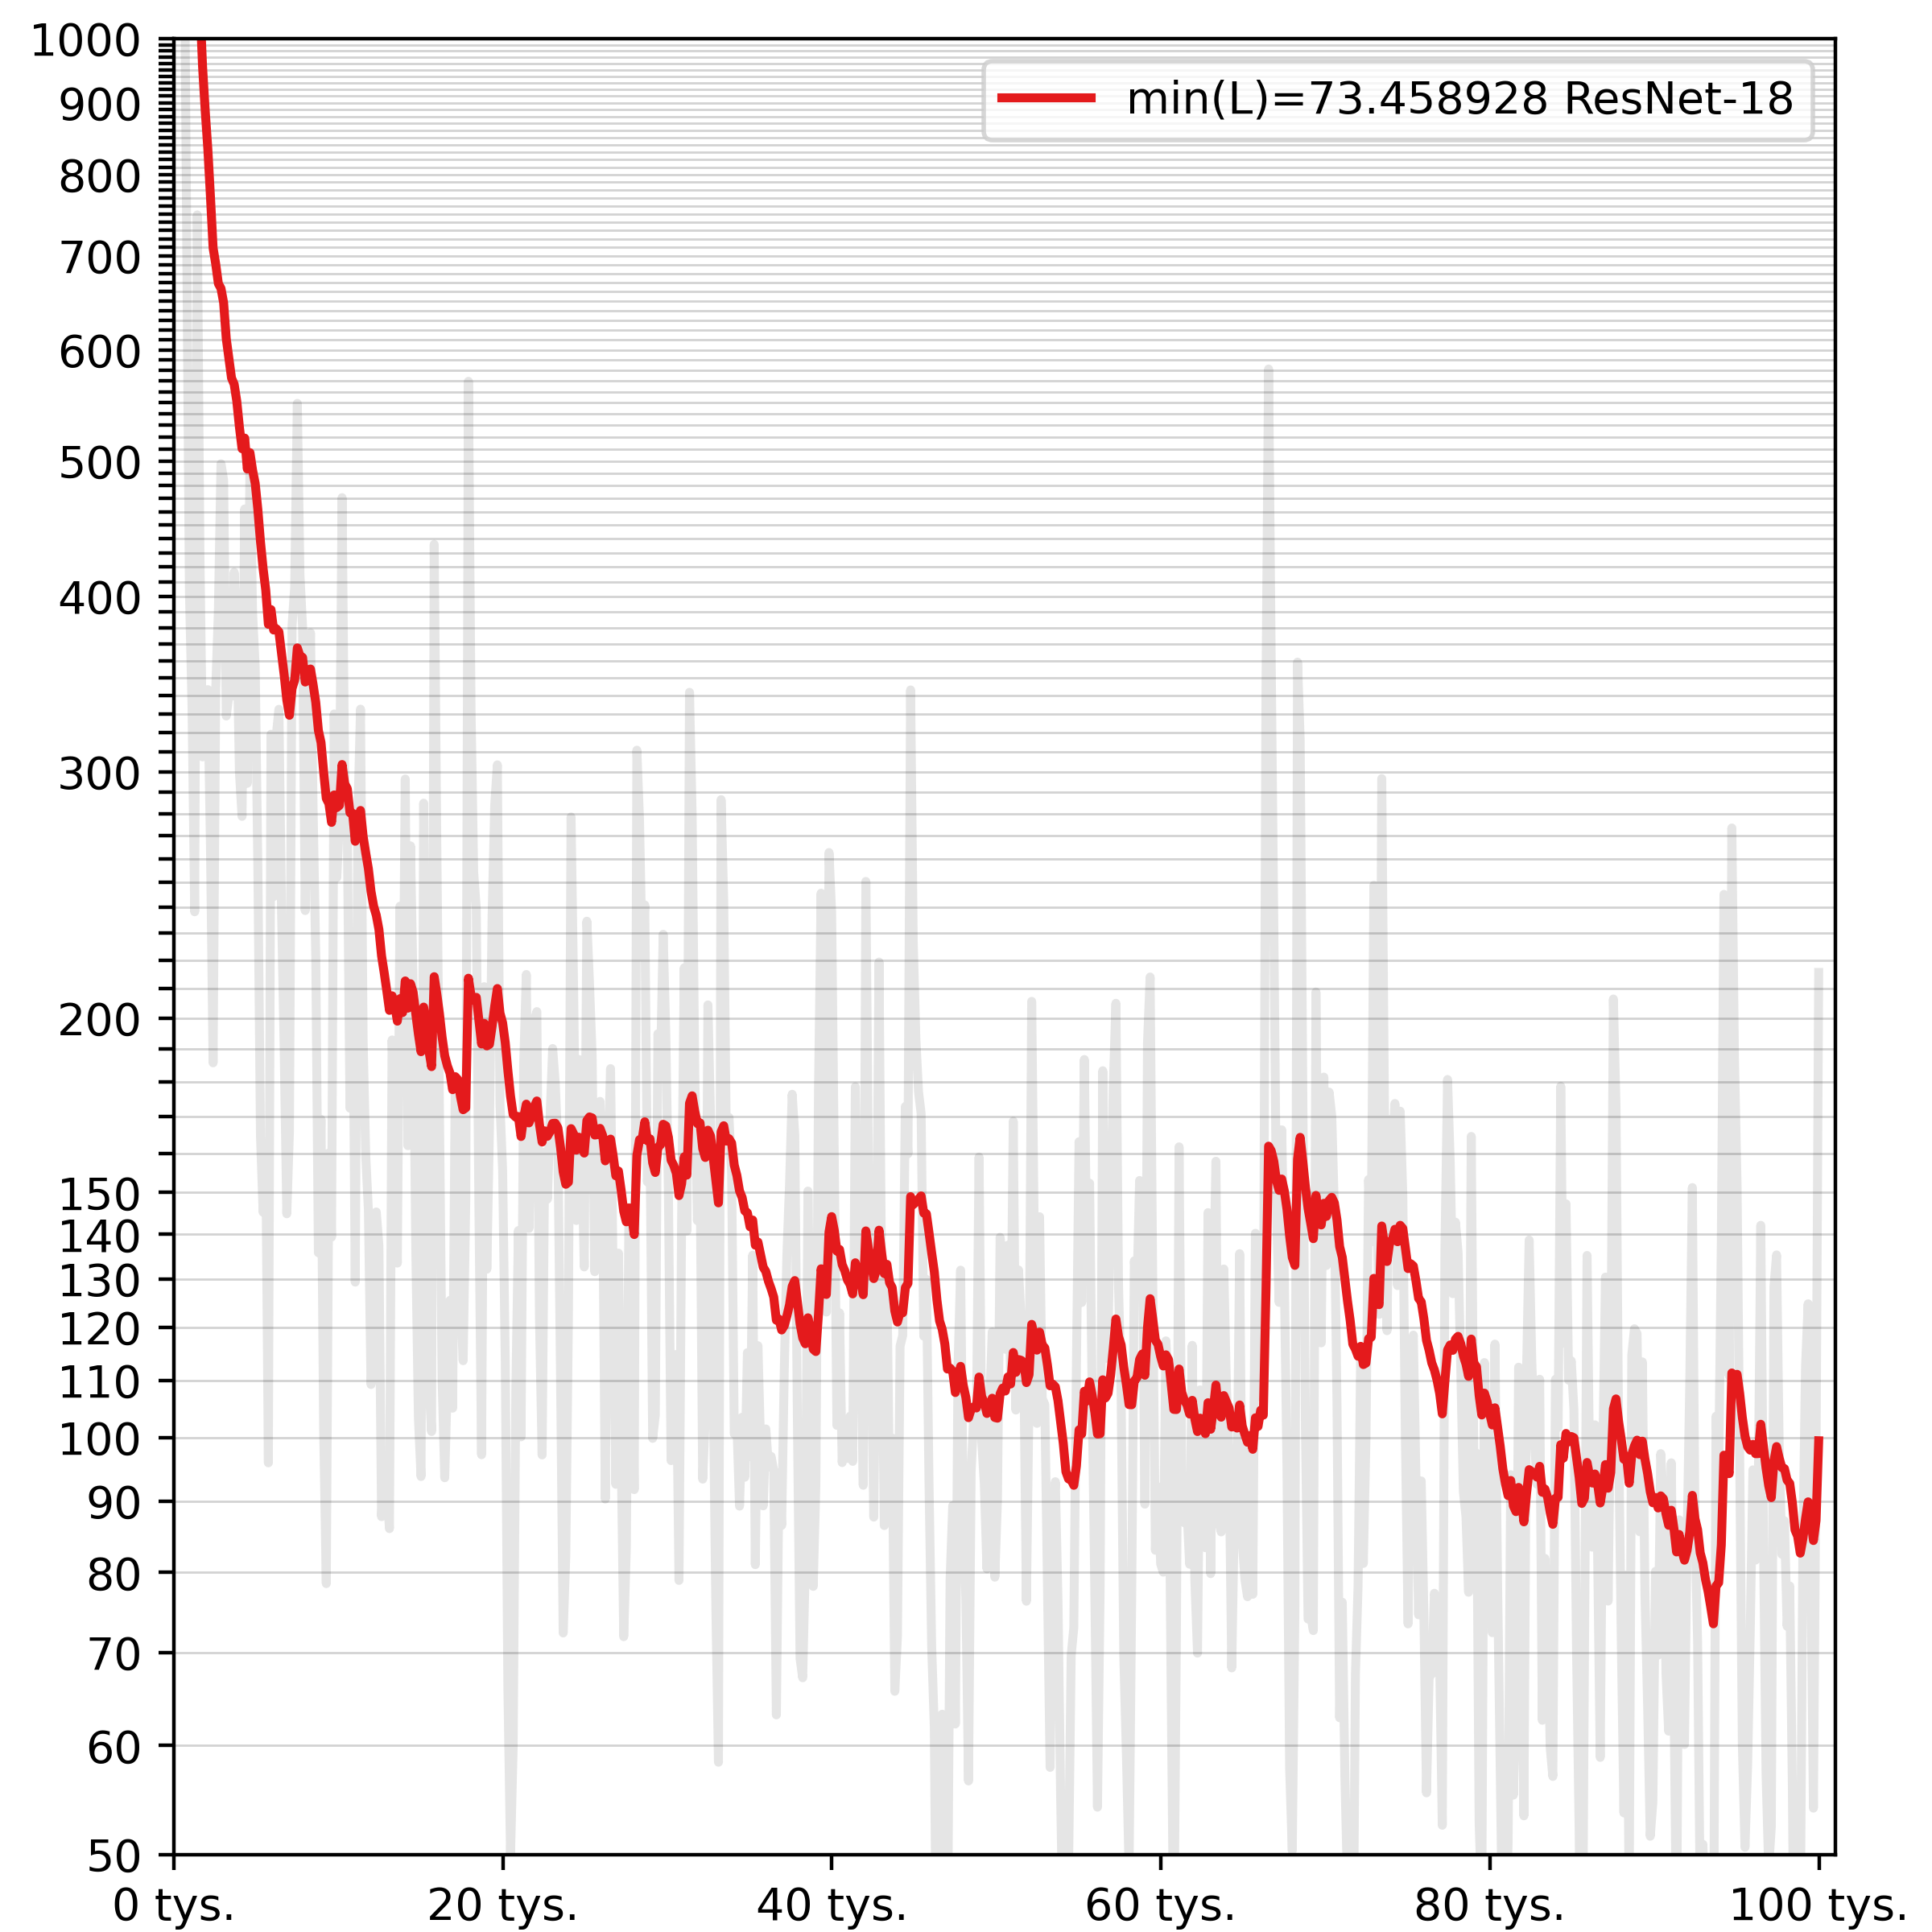
\includegraphics[width=0.47\linewidth]{determinism0.png} }}
    \qquad
    \subfloat[\centering Drugi przebieg trenowania]{{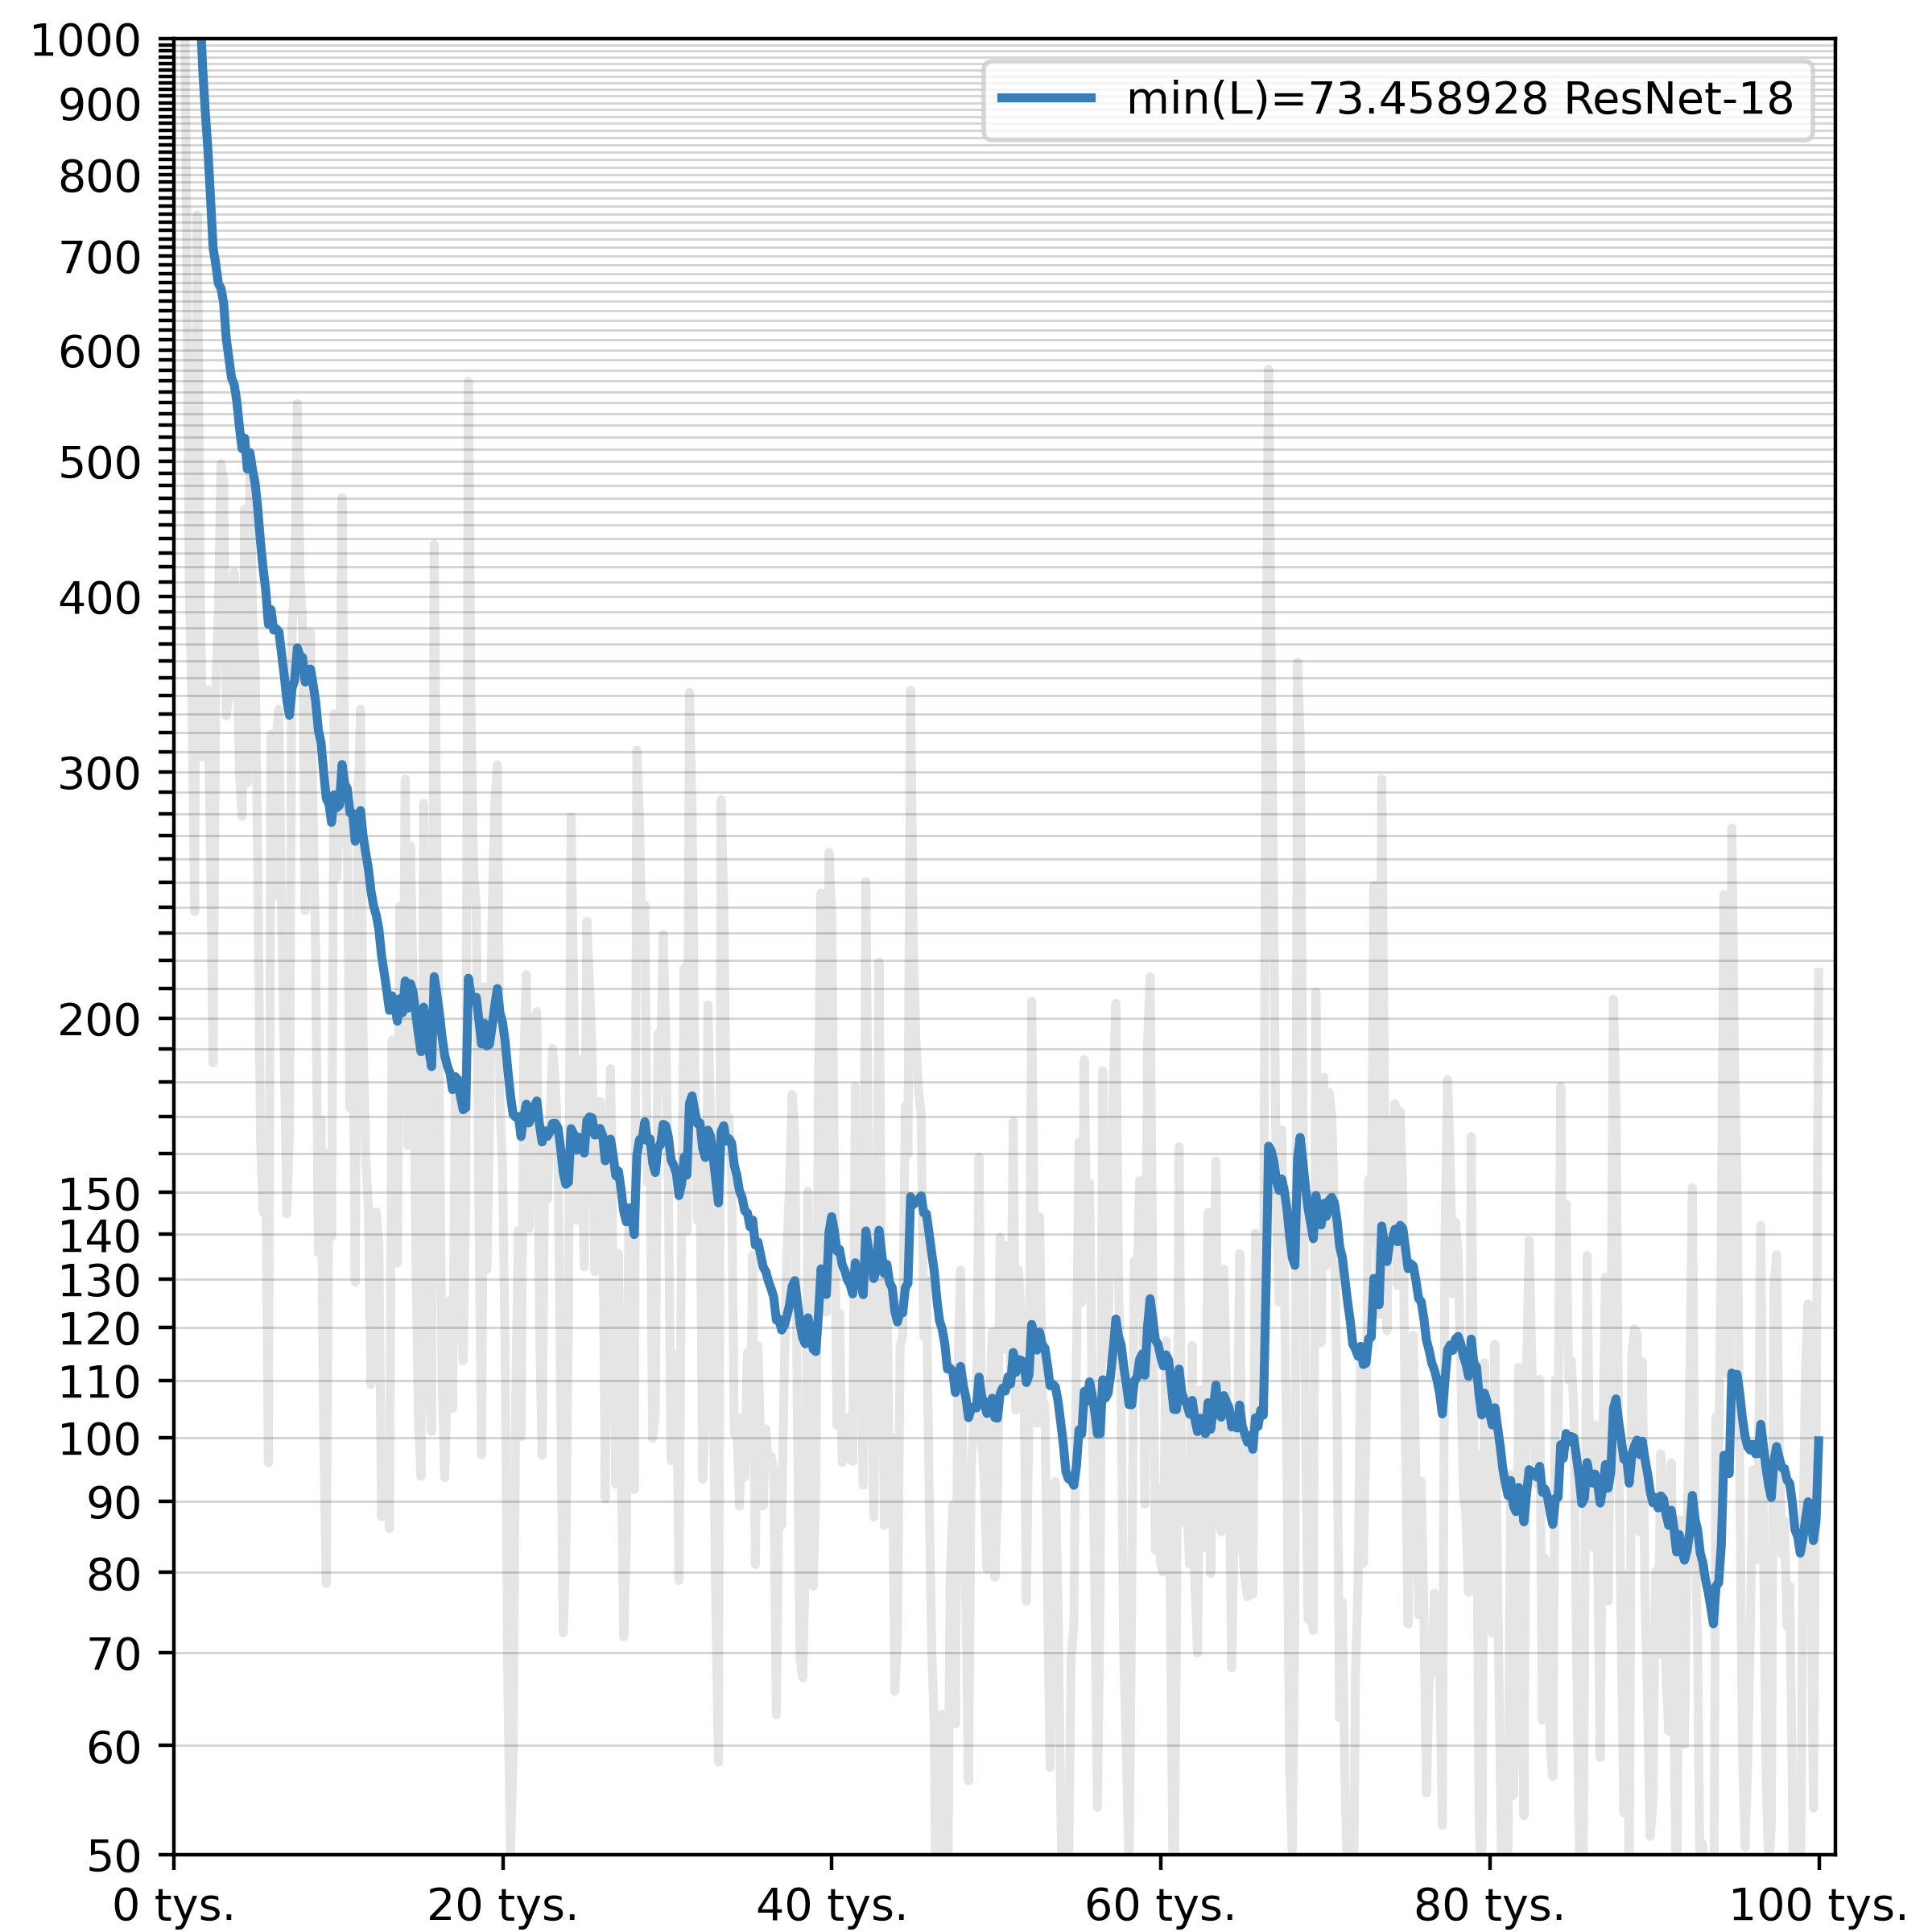
\includegraphics[width=0.47\linewidth]{determinism1.png} }}
\end{figure}

Wyniki uzyskane w dwóch przebiegach algorytmu trenującego są takie same (jak widać na powyższych rysunkach). Wartości funkcji kosztu są identyczne tzn. $|L_0(iter) - L_1(iter)| = 0$. Dowodzi to prawidłowemu działaniu funkcji ustalającej determinizm w procesie trenowania sieci neuronowych.